% *******************************************************************************
% * Copyright (c) 2007 by Elexis
% * All rights reserved. This document and the accompanying materials
% * are made available under the terms of the Eclipse Public License v1.0
% * which accompanies this distribution, and is available at
% * http://www.eclipse.org/legal/epl-v10.html
% *
% * Contributors:
% *    G. Weirich - initial implementation
% *    
% *  $Id: laborview.tex 2441 2007-05-28 18:49:56Z rgw_ch $
% *******************************************************************************

\section{Laboranzeige-View}
Bei Elexis werden sowohl interne als auch externe Laborbefunde, sowohl
automatisch eingelesene als auch manuell eigegebene Befunde in derselben Sicht
angezeigt. 

Die  Anzeige eines Befundes wird bestimmt durch
\begin{itemize}
  \item Ein Laboritem, zu dem dieser Befund gehört
  \item Ein Datum, an dem dieser Befund erhoben wurde
  \item Einen Patienten, zu dem dieser Befund gehört
\end{itemize}

Das Laboritem definiert, wie und wo der Laborbefund angezeigt werden soll, und
zu welchem Typ von Laborwerten er gehört.
Das Laboritem hat daher folgende Eingenschaften:
\begin{itemize}
  \item Das Labor, von dem er stammt
  \item Referenzbereich, getrennt für Männer und Frauen
  \item Titel
  \item Abkürzung
  \item Gruppe
  \item Sortierfolge
\end{itemize}

Das Erstellen von Labritems ist in der Regel nur bei der Installation des
Programms notwendig, bzw. dann, wenn Sie neue Laborparameter in Ihre
Standardbesimmungen aufnehmen möchten.
Das genaue Vorgehen ist unter Konfiguration genauer beschrieben.

 %\usepackage{graphics} is needed for \includegraphics
\begin{figure}[htp]
\begin{center}
  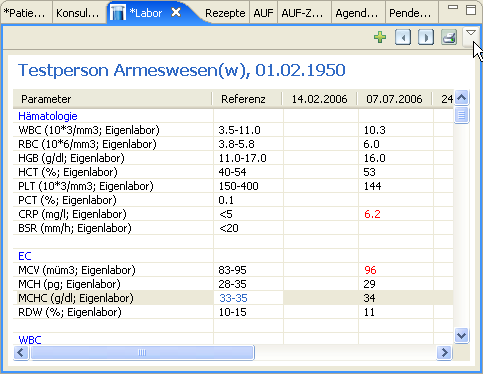
\includegraphics{images/labview}
  \caption{Labor-Anzeige}
  \label{fig:labview}
\end{center}
\end{figure}

Um Laborwerte manuell einzutragen, gehen Sie so vor:
\begin{itemize}
  \item Klicken Sie auf die Titelzeile der Tabelle. Es öffnet sich eine
  Dialogbox, n der Sie as Datum eingeben können.
\end{itemize}